\documentclass[a4paper, 14pt]{article}

\usepackage{arxiv}

\usepackage[T2A]{fontenc}
\usepackage[utf8]{inputenc}
\usepackage[english, russian]{babel}
% \usepackage{cmap}
\usepackage{url}
\usepackage{booktabs}
\usepackage{nicefrac}
\usepackage{microtype}
\usepackage{lipsum}
\usepackage{graphicx}
\usepackage{subfig}
\usepackage[square,sort,comma,numbers]{natbib}
\usepackage{doi}
\usepackage{multicol}
\usepackage{multirow}
\usepackage{tabulary}

\usepackage{tikz}
\usetikzlibrary{matrix}

% Algorithms
\usepackage{algpseudocode}
\usepackage{algorithm}

%% Шрифты
\usepackage{euscript} % Шрифт Евклид
\usepackage{mathrsfs} % Красивый матшрифт
\usepackage{extsizes} % Возможность сделать 14-й шрифт

\usepackage{makecell} % diaghead in a table
\usepackage{amsmath,amsfonts,amssymb,amsthm,mathtools,dsfont}
\usepackage{icomma}

\newcommand{\bz}{\mathbf{z}}
\newcommand{\bx}{\mathbf{x}}
\newcommand{\by}{\mathbf{y}}
\newcommand{\bv}{\mathbf{v}}
\newcommand{\bw}{\mathbf{w}}
\newcommand{\ba}{\mathbf{a}}
\newcommand{\bb}{\mathbf{b}}
\newcommand{\bff}{\mathbf{f}}
\newcommand{\bh}{\mathbf{h}}
\newcommand{\bl}{\mathbf{l}}
\newcommand{\bp}{\mathbf{p}}
\newcommand{\bq}{\mathbf{q}}
\newcommand{\bt}{\mathbf{t}}
\newcommand{\bu}{\mathbf{u}}
\newcommand{\bT}{\mathbf{T}}
\newcommand{\bX}{\mathbf{X}}
\newcommand{\bZ}{\mathbf{Z}}
\newcommand{\bS}{\mathbf{S}}
\newcommand{\bH}{\mathbf{H}}
\newcommand{\bW}{\mathbf{W}}
\newcommand{\bY}{\mathbf{Y}}
\newcommand{\bU}{\mathbf{U}}
\newcommand{\bQ}{\mathbf{Q}}
\newcommand{\bP}{\mathbf{P}}
\newcommand{\bA}{\mathbf{A}}
\newcommand{\bB}{\mathbf{B}}
\newcommand{\bC}{\mathbf{C}}
\newcommand{\bE}{\mathbf{E}}
\newcommand{\bF}{\mathbf{F}}
\newcommand{\bsigma}{\boldsymbol{\sigma}}
\newcommand{\bomega}{\boldsymbol{\omega}}
\newcommand{\btheta}{\boldsymbol{\theta}}
\newcommand{\bgamma}{\boldsymbol{\gamma}}
\newcommand{\bdelta}{\boldsymbol{\delta}}
\newcommand{\bPsi}{\boldsymbol{\Psi}}
\newcommand{\bpsi}{\boldsymbol{\psi}}
\newcommand{\bxi}{\boldsymbol{\xi}}
\newcommand{\bmu}{\boldsymbol{\mu}}
\newcommand{\bchi}{\boldsymbol{\chi}}
\newcommand{\bzeta}{\boldsymbol{\zeta}}
\newcommand{\blambda}{\boldsymbol{\lambda}}
\newcommand{\beps}{\boldsymbol{\varepsilon}}
\newcommand{\bZeta}{\boldsymbol{Z}}
% mathcal
\newcommand{\cX}{\mathcal{X}}
\newcommand{\cY}{\mathcal{Y}}
\newcommand{\cW}{\mathcal{W}}

\newcommand{\dH}{\mathds{H}}
\newcommand{\dR}{\mathds{R}}
% transpose
\newcommand{\T}{^{\mathsf{T}}}

% \renewcommand{\shorttitle}{\textit{arXiv} Шаблон}
\renewcommand{\epsilon}{\ensuremath{\varepsilon}}
\renewcommand{\phi}{\ensuremath{\varphi}}
\renewcommand{\kappa}{\ensuremath{\varkappa}}
\renewcommand{\le}{\ensuremath{\leqslant}}
\renewcommand{\leq}{\ensuremath{\leqslant}}
\renewcommand{\ge}{\ensuremath{\geqslant}}
\renewcommand{\geq}{\ensuremath{\geqslant}}
\renewcommand{\emptyset}{\varnothing}

\usepackage{hyperref}
% \usepackage[usenames,dvipsnames,svgnames,table,rgb]{xcolor}

\hypersetup{
	unicode=true,
	pdftitle={A template for the arxiv style},
	pdfsubject={q-bio.NC, q-bio.QM},
	pdfauthor={David S.~Hippocampus, Elias D.~Striatum},
	pdfkeywords={First keyword, Second keyword, More},
	colorlinks=true,
	linkcolor=black,        % внутренние ссылки
	citecolor=blue,         % на библиографию
	filecolor=magenta,      % на файлы
	urlcolor=blue           % на URL
}

\graphicspath{{../figures/}}

\usepackage{enumitem} % Для модификаций перечневых окружений

\theoremstyle{definition} % "Определение"
\newtheorem{definition}{Опр.}[section]

\usepackage{etoolbox}

\makeatletter
\expandafter\patchcmd\csname\string\algorithmic\endcsname{\itemsep\z@}{\itemsep=1.5mm}{}{}
\makeatother
\renewcommand{\abstractname}{Аннотация}

\title{Способы учёта шума данных в модели нейронных дифференциальных уравнений}

\author{Владимиров Эдуард \\
	\texttt{vladimirov.ea@phystech.edu} \\
	
	\And
	Стрижов Вадим \\
	\texttt{strijov@phystech.edu}
}
\date{\today}

\begin{document}
	\maketitle
	
	\begin{abstract}
		TODO
	\end{abstract}
	
	\keywords{временной ряд \and нейронные обыкновенные дифференциальные уравнения \and нейронные стохастические дифференциальные уравнения \and шум}
	
	\section{Введение}
	Извлечение шума является важной частью предобработки данных, так как он ограничивает процесс извлечения информации. 
	Для того, чтобы нивелировать эффект зашумлённости данных на качество предсказательной модели, необходимо либо заранее предобработать временной ряд, либо внедрить в неё механизм очистки данных, например аугментации, либо, наоборот, добавить шум к чистым данным.
	
	Во многих случаях временные ряды создаются низкоразмерной динамической системой.
	Тогда загрязнение шумом временных рядов может привести к затруднению поиска оптимальной размерности эмбеддинга \cite{kostelich1990noise} и ограничению точности прогнозирования \cite{elshorbagy2002noise}. Поэтому снижение
	уровня шума при сохранении базовой динамики, генерируемой на основе временных рядов, имеет первостепенное значение.
	
	\begin{table}[bhtp]
		\caption{Классификация методов фильтрации временных рядов и их аналогов в фреймворке Neural ODE}
		\begin{tabulary}{\textwidth}{|C|C|C|}
			\hline
			\textbf{Механизм предобработки} & \textbf{Фильтры} & \textbf{Аналог в фреймворке NODE} 
			\\ \hline
			Разложение & вейвлет-преобразование, преобразование Фурье, метод главных компонент & --- 
			\\ \hline
			Итеративный со скрытой динамикой & фильтр Калмана & непрерывный процесс потока времени (Continuous Time Flow Process, CTFP) \cite{Deng2020}, GRU-ODE-Bayes \cite{DeBrouwer2020}
			\\ \hline
			Итеративный & экспоненциальное сглаживание, модель Хольта-Брауна, пакетная нормализация & ---
			\\ \hline
			Введение случайности & dropout, добавление гауссовского шума
			& NSDE с разными компонентами перед дифференциалом от стандартного броуновского движения \cite{Liu2019}
			\\ \hline
		\end{tabulary}
	\end{table}
	
	Существует несколько основных методов предобработки сигналов.
	Фильтр Калмана \cite{Dhwaj2018} использует информацию о физике самого явления.
	Вейвлет преобразование \cite{Alrumaih2002} раскладывает временной ряд на множество других с разным разрешением.
	Экспоненциальное сглаживание \cite{gardner1985exponential} выравнивает временной ряд с помощью экспоненциальной оконной функции.
	В работе \cite{Ignatov2016} фильтрация одномерного временного ряда выполняется в несколько этапов.
	Вначале строится матрица Ханкеля на основе теоремы Такенса \cite{noakes1991takens}.
	Затем выполняется сингулярное разложение этой матрицы с сохранением некоторого числа первых компонент.
	После этого исходный ряд восстанавливается как среднее значение элементов на побочных диагоналях.
	
	Модель нейронных дифференциальных уравнений (Neural Ordinary Differential Equation, NODE) \cite{Chen2018} объединяет в себе нейронные сети и дифференциальные уравнения. 
	Помимо использования в моделировании динамических системах, она также применяется в задачах интерполяции, экстраполяции и генерации временных рядов, в частности в финансах, робототехнике \cite{xie2019neural, meleshkova2021application, du2020model}. 
	Данный механизм является непрерывным аналогом сети ResNet \cite{wu2019wider}, в которой впервые использовались остаточные соединения для решения проблемы затухающих градиентов.
	NODE объединяет в себе плюсы из обоих миров. 
	Структура нейронной сети даёт высокую обобщающую способность, а структура дифференциального уравнения даёт твёрдый теоретический фундамент.
	Однако у этого фреймворка есть и минусы. 
	Существует класс функций, которые не представимы этой моделью \cite{Dupont2019}, а также она плохо устойчива к шуму в данных \cite{Liu2019}.
	
	Для решения вышеизложенных проблем было разработано новое семейство нейронных сетей ~--- стохастические дифференциальные уравнения (Neural Stochastic Differential Equation, NSDE).
	Она внедряет шум в модель NODE с помощью стохастического дифференциального уравнения (SDE).
	Данный фреймворк позволяет эксплуатировать такие регуляризаторы, как Dropout и слой гауссовского шума \cite{liu2018towards, baldi2013understanding}.
	Однако остаётся вопрос: можно ли внедрить другие регуляризаторы (например, BatchNorm) и вышеупомянутые методы фильтрации в фреймворк NODE? 
	В данной работе планируется ответить на этот вопрос.
	
	[TODO: Краткое описание вычислительного эксперимента]
	
	\section{Сопутствующие работы}
	Наша работа вдохновлена успехом модели Neural ODE и её многочисленных модификаций: ANODE, Neural SDE, Neural CDE.
	Мы стремимся перенести некоторые методы фильтрации временных рядов в модель нейронных дифференциальных уравнений.
	Однако такие регуляризаторы, как пакетная нормализация и вейвлет преобразование, тяжело внедрить в Neural ODE ввиду отсутствия скрытой динамики.

	\subsection{Neural ODE}
	Как было сказано ранее, модель нейронных дифференциальных уравнений является непрерывным расширением модели ResNet, в которой параметризуется производная скрытого состояния.
	\begin{equation*} \label{eq:resnet_step}
		\bh_{t+1} = \bh_t + f_{\theta_t}(\bh_t).
	\end{equation*}
	Разность $\bh_{t+1} - \bh_t$ можно интерпретировать как дискретизацию производной $\bh'(t)$ c разницей во времени $\Delta t = 1$. Устремив $\Delta t \rightarrow 0$, получим:
	\begin{equation*} \label{eq:node}
		\lim_{\Delta t \rightarrow 0} \dfrac{\bh_{t + \Delta t} - \bh_t}{\Delta t} = \dfrac{d\bh(t)}{dt} = f_{\theta}(\bh(t), t)
	\end{equation*}
	Модель нейронных дифференциальных уравнений аппроксимирует отображение $\bx \rightarrow \by$ путём обучения нейронной сети $f_\theta$ и линейных отображений $l_\theta^1, \, l_\theta^2$.
	$$ \by \approx l_\theta^2(\bh_T), \text{ где } \bh_T = \bh_0 + \int_{0}^{T} f_\theta(\bh_t) dt \text{ и } \bh_0 = l_\theta^1(\bx)$$
	
	\subsection{Neural SDE}
	Конструкция выглядит следующим образом.
	Зафиксируем момент времени $T > 0$.
	Обозначим за $(\bY_t, t \in [0, T]$ искомый $y$-мерный случайный процесс, где $y$ ~--- размерность данных.
	
	Пусть $(\bW_t, t \in [0, T])$  ~--- $w$-мерный винеровский процесс и $V \sim \mathcal{N}(0, I_v)$ ~--- $v$-мерный стандартный гауссовский вектор. 
	Пусть
	$$ \zeta_\theta: \dR^v \rightarrow \dR^d, \; \mu_\theta: [0, T] \times \dR^d \rightarrow \dR^d, \; \sigma_\theta: [0, T] \times \dR^d \rightarrow \dR^{d \times w}, \; l_\theta: \dR^d \rightarrow \dR^y,$$
	где $d$ ~--- размерность скрытого состояния, $\zeta_\theta, \mu_\theta, \sigma_\theta$ ~--- нейронные сети, $l_\theta$ ~--- линейное преобразование.
	Тогда модель Neural SDE имеет следующий вид:  
	$$ \bh_0 = \zeta_\theta(V), \quad d\bh_t = \mu_\theta(t, \bh_t)dt + \sigma_\theta(t, \bh_t) \circ d\bW_t, \quad \widehat{\bY_t} = l_\theta(\bh_t).$$
	Решением SDE служит случайный $d$-мерный процесс $(\bh_t, t \in [0, T])$.
	Модель обучается таким образом, что $\widehat{\bY} \approx \bY$
	
	В работе \cite{Liu2019} показано, что добавление гауссовского шума выражается следующим образом: $\sigma(t, \bh_t) = \Sigma(t), \:$ где $\Sigma(t)$ ~--- диагональная матрица с элементами, отвечающими за дисперсию шума, добавляемого к вектору скрытого состояния.
	А слой Dropout представляется так: $\sigma(t, \bh_t) = \sqrt{\dfrac{1 - p}{p}} \mu_\theta(t, \bh_t)$, где $p$ ~--- вероятность успеха в схеме испытаний Бернулли. 
	
	\subsection{ResNet}
	Нетрудно заметить, что блок \ref{eq:resnet_step} модели ResNet соответствует одному шагу метода Эйлера численного интегрирования уравнения \ref{eq:node}.
	Учитывая этот факт и то, что существует множество регуляризаторов для данного семейства моделей: DropBlock, Shake-Shake [TODO: ссылки]; хочется найти их аналоги для фреймворка Neural ODE.
	
	\section{Постановка задачи}
	Общая схема данных в задаче удаления шума имеет вид:  
	$$\bx_t = \bs_t + \boldsymbol{\epsilon_t},$$
	где $\bx_t$ ~--- наблюдаемое значение временного ряда, $\boldsymbol{\epsilon_t}$ ~--- многомерный винеровский процесс, $\bs_t$ ~--- истинное значение временного ряда.
	Задача удаления шума заключается в подавлении шумовой составляющей временного ряда $\bx_t$ и восстановлении $\bs_t$.
	
	\section{Вычислительный эксперимент}
	Сначала покажем, что качество модели Neural ODE уменьшается при наличии шума в данных.
	Взят синтетический временной ряд "Спираль", и его зашумлённый вариант с добавленным нормальным шумом $\mathcal{N}(0, 0.04^2)$ ( график \ref{fig:spirals}).
	
	\begin{figure}[bhtp]
		\centering
		\subfloat[Временной ряд "Спираль"]{%
			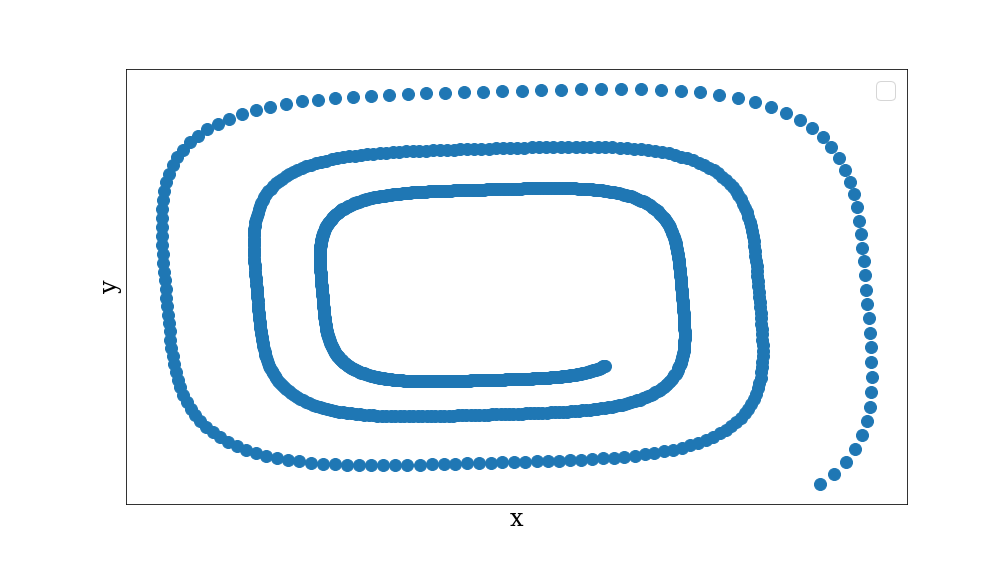
\includegraphics[width=0.48\linewidth]{Spirals.png}%
		}
		\subfloat[Зашумлённая спираль]{%
			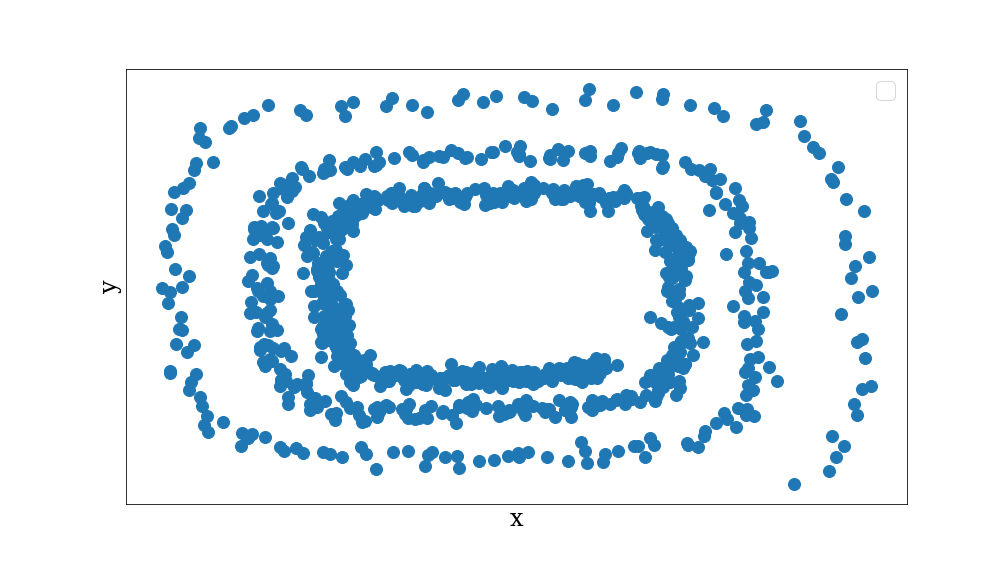
\includegraphics[width=0.48\linewidth]{Noisy spirals.png}
		}
		\caption{Синтетические данные}
		\label{fig:spirals}
	\end{figure}

	Результат применения модели Neural ODE и графики функции потерь при обучении приведены на графиках \ref{fig:spirals_approximation} и \ref{fig:train_losses}.
	
	\begin{figure}[bhtp]
		\centering
		\subfloat[NODE на чистых данных]{%
			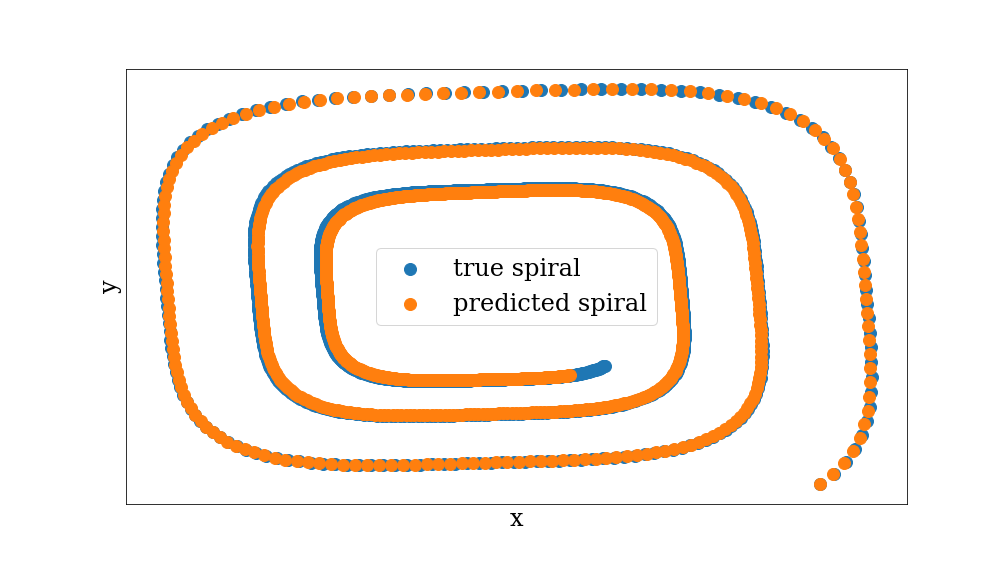
\includegraphics[width=0.5\linewidth]{Spirals vs ODE Spirals.png}%
		}
		\subfloat[NODE на зашумлённых данных]{%
			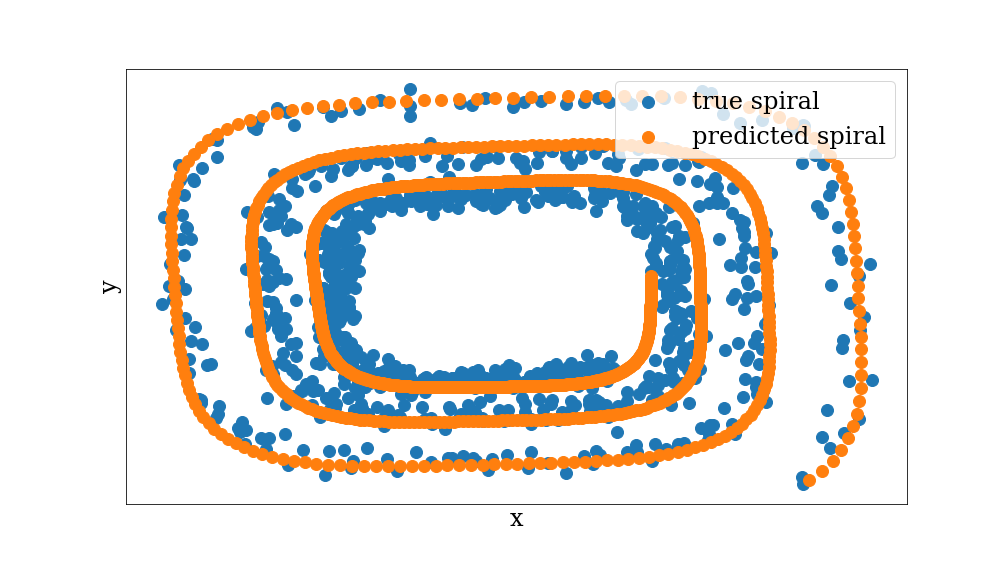
\includegraphics[width=0.5\linewidth]{Noisy Spirals vs ODE Spirals.png}
		}
		\caption{Результаты предсказания}
		\label{fig:spirals_approximation}
	\end{figure}
	
	\begin{figure}[bhtp]
		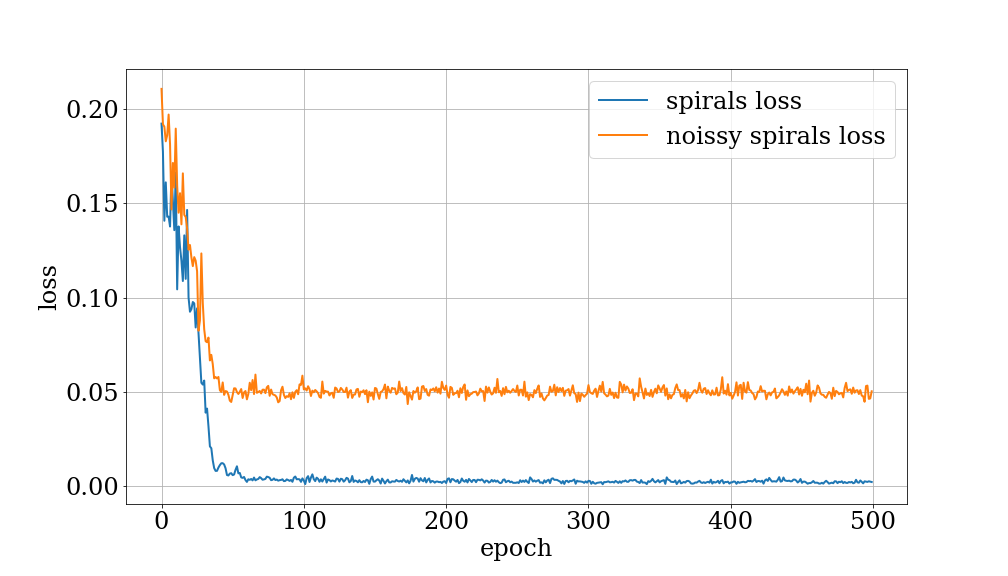
\includegraphics[width=0.95\linewidth]{train_losses.png}
		\caption{Функция потерь при обучении Neural ODE на незашумлённых и зашумлённых данных}
		\label{fig:train_losses}
	\end{figure}
	
	\section{Заключение}
	TODO
	
	\bibliographystyle{unsrtnat}
	\bibliography{references.bib}
	
\end{document}